\documentclass[10pt,aspectratio=169]{beamer}
\usetheme{Frankfurt}
\usecolortheme{seahorse}
\setbeamertemplate{navigation symbols}{}
\setbeamertemplate{footline}[frame number]

\usepackage[a4paper,margin=1cm]{geometry}
\usepackage{amsmath,amssymb,amsthm}
\usepackage{booktabs}
\usepackage{xcolor}
\usepackage{tikz}
\usetikzlibrary{positioning,arrows.meta}
\usepackage{enumitem}
\usepackage{hyperref}
\hypersetup{colorlinks=true,linkcolor=blue!60!black}
\usepackage{caption}
\usepackage{subcaption}
\usepackage{verbatim}
\usepackage{listings}
\renewcommand{\familydefault}{\sfdefault}

% TikZ styles (copied from original)
\tikzset{
  nd/.style={circle, fill=white, draw=black, minimum size=12pt, thick},
  term/.style={circle, fill=gray!40, draw=black, minimum size=10pt, thick},
  Lleaf/.style={circle, fill=blue!20, draw=blue, minimum size=10pt, thick},
  Rleaf/.style={circle, fill=red!20, draw=red, minimum size=10pt, thick},
  Le/.style={draw=blue!70, line width=2pt, ->,>=stealth},
  Re/.style={draw=red!70, line width=2pt, ->,>=stealth},
  lbl/.style={font=\tiny\bfseries, inner sep=1pt},
  gametree/.style={scale=1}
}

% Colours (copied from original)
\definecolor{lblue}{RGB}{55,138,221}
\definecolor{rred}{RGB}{226,75,74}

% Macros (copied from original)
\newcommand{\Lopt}[1]{{\color{lblue}\textbf{#1}}}
\newcommand{\Ropt}[1]{{\color{rred}\textbf{#1}}}
\newcommand{\Gv}[1]{\mathcal{G}(#1)}
\newcommand{\tmp}[1]{t\!\left(#1\right)}

\title{Leaf Convergence Games:\\ Partizan Games on Terminating Rooted Graphs}
\subtitle{IE619 --- Combinatorial Game Theory (2025)}
\author{Your Name / Presenter}
\date{\today}

\begin{document}

% ==================== TITLE SLIDE ====================
\begin{frame}
  \maketitle
  \begin{center}
    \Large A new class of partizan games with guaranteed termination
  \end{center}
\end{frame}

% ==================== ABSTRACT ====================
\begin{frame}{Abstract}
  We introduce \textbf{Leaf Convergence Games (LCG)}, a partizan combinatorial game played on finite rooted graphs whose edges are labelled \Lopt{L} (blue) or \Ropt{R} (red), with the key structural constraint that \textbf{all maximal paths terminate at designated terminal nodes}.

  \vspace{10pt}
  A token starts at the root. \Lopt{Left} moves along \Lopt{L}-edges and \Ropt{Right} along \Ropt{R}-edges. The player unable to move loses (normal play).

  \vspace{10pt}
  \textbf{Key properties:}
  \begin{itemize}
    \item All games terminate in finite time (no cycles).
    \item Leaf structure completely determines endgame strategy.
    \item Rich game values: integers, switches, infinitesimals, dyadic rationals.
  \end{itemize}

  Exhaustive computational analysis performed with a custom Python evaluator and CGSuite.
\end{frame}

% ==================== INTRODUCTION ====================
\begin{frame}{Introduction}
  \textbf{Leaf Convergence Games (LCG)} are partizan games on finite rooted DAGs with the convergence property:
  \begin{itemize}
    \item Every maximal path from the root ends at a terminal node $\tau \in \mathcal{T}$ (no outgoing edges).
    \item Edges labelled \Lopt{L} (blue) or \Ropt{R} (red).
    \item Token starts at root; Left moves on blue, Right on red.
  \end{itemize}

  \vspace{15pt}
  \textbf{Why this class is interesting:}
  \begin{itemize}
    \item \textbf{Termination guarantee} — no loops, always finite play.
    \item \textbf{Topology-agnostic} — linear, branched, multi-sink, arbitrary DAGs.
    \item \textbf{Strategic depth} — branching + asymmetry creates rich CGT values.
  \end{itemize}

  Unlike standard impartial games or loopy games, LCGs are always well-founded.
\end{frame}

% ==================== MOTIVATING STRUCTURES ====================
\begin{frame}{Motivating Structures}
  \begin{columns}
    \begin{column}{0.33\textwidth}
      \centering
      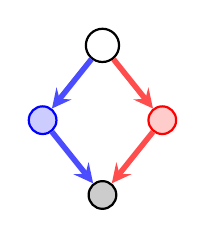
\begin{tikzpicture}[gametree, scale=0.95]
        \node[nd] (r) at (0,0) {};
        \node[Lleaf] (l) at (-0.8,-1.0) {};
        \node[Rleaf] (r1) at (0.8,-1.0) {};
        \node[term] (t) at (0,-2.0) {};
        \draw[Le] (r)--(l); \draw[Re] (r)--(r1);
        \draw[Le] (l)--(t); \draw[Re] (r1)--(t);
      \end{tikzpicture}
      \small Linear convergence: simple star
    \end{column}
    \begin{column}{0.33\textwidth}
      \centering
      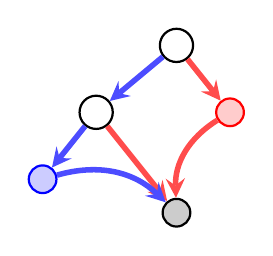
\begin{tikzpicture}[gametree, scale=0.85]
        \node[nd] (r) at (0,0) {};
        \node[nd] (l1) at (-1.2,-1.0) {};
        \node[Rleaf] (l2) at (0.8,-1.0) {};
        \node[Lleaf] (l3) at (-2.0,-2.0) {};
        \node[term] (t) at (0,-2.5) {};
        \draw[Le] (r)--(l1); \draw[Re] (r)--(l2);
        \draw[Le] (l1)--(l3); \draw[Re] (l1)--(t);
        \draw[Re] (l2) to[bend right] (t);
        \draw[Le] (l3) to[bend left] (t);
      \end{tikzpicture}
      \small Mixed depth + early termination
    \end{column}
    \begin{column}{0.33\textwidth}
      \centering
      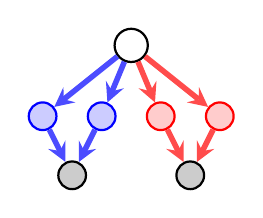
\begin{tikzpicture}[gametree, scale=0.75]
        \node[nd] (r) at (0,0) {};
        \node[Lleaf] (l1) at (-1.5,-1.2) {};
        \node[Lleaf] (l2) at (-0.5,-1.2) {};
        \node[Rleaf] (r1) at (0.5,-1.2) {};
        \node[Rleaf] (r2) at (1.5,-1.2) {};
        \node[term] (t1) at (-1.0,-2.2) {};
        \node[term] (t2) at (1.0,-2.2) {};
        \draw[Le] (r)--(l1); \draw[Le] (r)--(l2);
        \draw[Re] (r)--(r1); \draw[Re] (r)--(r2);
        \draw[Le] (l1)--(t1); \draw[Le] (l2)--(t1);
        \draw[Re] (r1)--(t2); \draw[Re] (r2)--(t2);
      \end{tikzpicture}
      \small Multi-sink convergence
    \end{column}
  \end{columns}
\end{frame}

% ==================== FORMAL DEFINITION ====================
\begin{frame}{Formal Framework}
  \textbf{LCG Position:}
  \begin{itemize}
    \item Finite directed acyclic graph (DAG) with root $r$ and terminal set $\mathcal{T}$.
    \item Every edge labelled \Lopt{L} or \Ropt{R}.
    \item \textbf{Convergence property:} Every maximal path from $r$ ends in some $\tau \in \mathcal{T}$.
  \end{itemize}

  \vspace{15pt}
  \textbf{Recursive Value (standard CGT notation):}
  \[
  \Gv{v} = \bigl\{ \Gv{c} : c \in \mathcal{L}(v) \;\big|\; \Gv{c} : c \in \mathcal{R}(v) \bigr\}
  \]
  where $\Gv{\tau} = 0$ for every terminal node $\tau$.

  \vspace{10pt}
  Game value is determined \textbf{entirely by branching structure and Left/Right asymmetry} — all leaves are 0.
\end{frame}

% ==================== DEPTH-1 VALUES ====================
\begin{frame}{Depth-1 Values}
  \textbf{Key Insight:} All leaves converge to value 0. Value arises purely from number of Left vs.\ Right options.

  \begin{table}
    \centering
    \small
    \begin{tabular}{@{}llllc@{}}
      \toprule
      Left & Right & CGSuite Code & Value & Temp \\
      \midrule
      1 & 0 & \texttt{\{0|\}} & 1 & $-\infty$ \\
      2 & 0 & \texttt{\{\{0|\}|\}} & 2 & $-\infty$ \\
      0 & 1 & \texttt{\{|0\}} & $-1$ & $-\infty$ \\
      0 & 2 & \texttt{\{\{|0\}|\}} & $-2$ & $-\infty$ \\
      1 & 1 & \texttt{\{0|0\}} & $*$ & 0 \\
      $n$ & $n$ & \texttt{\{0|0\}} & $*$ & 0 \\
      1 & 2 & \texttt{\{1|-1\}} & $\pm 1$ & 1 \\
      2 & 1 & \texttt{\{2|-2\}} & $\pm 2$ & 2 \\
      \bottomrule
    \end{tabular}
  \end{table}

  Pure integers, star, and switches appear already at depth 1.
\end{frame}

% ==================== STRUCTURAL THEOREMS ====================
\begin{frame}{Structural Theorems}
  \begin{theorem}[Termination Guarantee]
    Every LCG terminates in finite time.
  \end{theorem}
  \begin{proof}
    Rank of node = longest path to any terminal. Ranks strictly decrease along every move.
  \end{proof}

  \begin{theorem}[Linear Convergence]
    All leaves converge to a common terminal $\implies$ value simplifies to $\{0,0,\dots | 0,0,\dots\}$.
  \end{theorem}

  \begin{theorem}[Multi-Sink Decomposition]
    Disjoint terminal sets $\implies$ value is disjunctive sum of subgames.
  \end{theorem}

  \begin{theorem}[Depth-$d$ Characterisation]
    \begin{itemize}
      \item Depth 1 $\to$ integers and switches.
      \item Depth 2 $\to$ dyadic rationals + infinitesimals.
      \item Depth $3+$ $\to$ arbitrarily rich CGT values.
    \end{itemize}
  \end{theorem}
\end{frame}

% ==================== EXAMPLE 1 ====================
\begin{frame}{Example 1: Asymmetric Depth Tree}
  \centering
  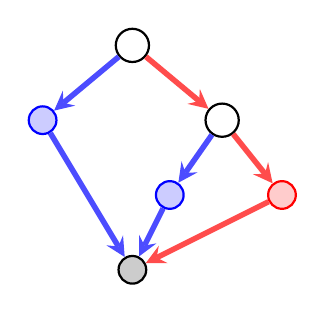
\begin{tikzpicture}[gametree, scale=0.95]
    \node[nd] (r) at (0,0) {};
    \node[Lleaf] (l) at (-1.2,-1.0) {};
    \node[nd] (rm) at (1.2,-1.0) {};
    \node[Lleaf] (rm_l) at (0.5,-2.0) {};
    \node[Rleaf] (rm_r) at (2.0,-2.0) {};
    \node[term] (t) at (0,-3.0) {};
    \draw[Le] (r)--(l); \draw[Re] (r)--(rm);
    \draw[Le] (rm)--(rm_l); \draw[Re] (rm)--(rm_r);
    \draw[Le] (l)--(t); \draw[Le] (rm_l)--(t);
    \draw[Re] (rm_r)--(t);
  \end{tikzpicture}

  \vspace{10pt}
  \textbf{Value Analysis:}
  \begin{itemize}
    \item Left option: direct leaf $\to 0$.
    \item Right option: subtree $\{0|0\} = *$.
    \item Root value: $\{0 \mid *\} = \uparrow$ (infinitesimal up).
  \end{itemize}
\end{frame}

% ==================== EXAMPLE 2 ====================
\begin{frame}{Example 2: Multi-Sink DAG}
  \centering
  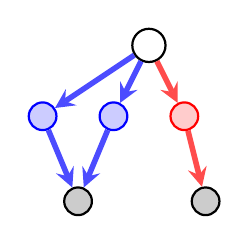
\begin{tikzpicture}[gametree, scale=0.9]
    \node[nd] (r) at (0,0) {};
    \node[Lleaf] (l1) at (-1.5,-1.0) {};
    \node[Lleaf] (l2) at (-0.5,-1.0) {};
    \node[Rleaf] (r1) at (0.5,-1.0) {};
    \node[term] (tl) at (-1.0,-2.2) {};
    \node[term] (tr) at (0.8,-2.2) {};
    \draw[Le] (r)--(l1); \draw[Le] (r)--(l2);
    \draw[Re] (r)--(r1);
    \draw[Le] (l1)--(tl); \draw[Le] (l2)--(tl);
    \draw[Re] (r1)--(tr);
  \end{tikzpicture}

  \vspace{10pt}
  \textbf{Value Analysis:}
  \begin{itemize}
    \item Both Left options $\to t_L$ (value 0).
    \item Right option $\to t_R$ (value 0).
    \item Root value: $\{0 \mid 0\} = *$.
  \end{itemize}
\end{frame}

% ==================== COMPUTATIONAL ANALYSIS ====================
\begin{frame}{Computational Analysis}
  \textbf{Python Recursive Evaluator (core snippet):}
  \begin{verbatim}
def evaluate_lcg(nodes, edges, root, terminals):
    memo = {}
    def eval_node(v):
        if v in terminals: return ([], [])
        left_opts = [eval_node(c) for ... if L-edge]
        right_opts = [eval_node(c) for ... if R-edge]
        return (left_opts, right_opts)
    return eval_node(root)
  \end{verbatim}

  \vspace{10pt}
  \textbf{CGSuite Verification:}
  \begin{itemize}
    \item Integers, switches, infinitesimals, atomic weights, temperatures all verified.
    \item Composite sums: $\pm 1 + *$, $\uparrow + \downarrow$, etc.
  \end{itemize}
\end{frame}

% ==================== VALUE ENUMERATION ====================
\begin{frame}{Value Enumeration Results (Depth 1--2)}
  \begin{table}
    \centering
    \small
    \begin{tabular}{@{}llrrr@{}}
      \toprule
      Configuration & Value & Temperature & Atomic Weight & Count \\
      \midrule
      Pure Left ($n$ leaves) & $n$ & $-\infty$ & $n$ & 5 \\
      Pure Right ($n$ leaves) & $-n$ & $-\infty$ & $-n$ & 5 \\
      Symmetric ($n$ L-R pairs) & $*$ & 0 & 0 & 5 \\
      Switches $\{n|-m\}$ & $\pm\min(n,m)$ & $\min(n,m)$ & varies & 15 \\
      Infinitesimal up $\{0|*\}$ & $\uparrow$ & 0 & $\uparrow$ & 1 \\
      Infinitesimal down $\{*|0\}$ & $\downarrow$ & 0 & $\downarrow$ & 1 \\
      \bottomrule
    \end{tabular}
  \end{table}
\end{frame}

% ==================== TEMPERATURE ANALYSIS ====================
\begin{frame}{Temperature Analysis}
  Temperature = incentive to move.

  \begin{itemize}
    \item \textbf{Frozen games} ($t(G)=-\infty$): Pure integers — one player dominates.
    \item \textbf{Cold games} ($t(G)=0$): Fuzzy games and infinitesimals — neither player is urgent.
    \item \textbf{Hot games} ($t(G)>0$): Switches — both players want to move first.
  \end{itemize}

  \vspace{15pt}
  Depth-$d$ behaviour:
  \begin{itemize}
    \item Depth 1: integers + switches.
    \item Depth 2: introduces dyadic rationals and infinitesimals ($\uparrow$, $\downarrow$).
    \item Deeper trees $\to$ arbitrarily rich temperature spectra.
  \end{itemize}
\end{frame}

% ==================== KEY TAKEAWAYS ====================
\begin{frame}{Key Takeaways}
  \begin{enumerate}
    \item \textbf{Termination is fundamental:} Acyclic convergence guarantees finite play.
    \item \textbf{Topology matters:} Linear, branched, and multi-sink structures produce distinct value classes.
    \item \textbf{Depth-$d$ completeness:} Depth-3 trees already realise rich CGT values.
    \item \textbf{Symmetry $\implies$ value 0:} Balanced L/R positions are always $*$.
    \item Leaf Convergence Games realise integers, switches, infinitesimals, and dyadic rationals with deep strategic tension.
  \end{enumerate}
\end{frame}

% ==================== OPEN QUESTIONS ====================
\begin{frame}{Open Questions}
  \begin{enumerate}[label=(\roman*)]
    \item Closed-form characterisation for arbitrary DAG topologies.
    \item Complete enumeration of all depth-3 position values.
    \item Efficient optimal strategy computation for large positions.
    \item Generalisation to fuzzy games and other play conventions.
    \item Connections to existing CGT value hierarchies.
  \end{enumerate}
\end{frame}

% ==================== REFERENCES ====================
\begin{frame}{References}
  \begin{thebibliography}{5}
    \setbeamertemplate{bibliography item}{\insertbiblabel}
    \bibitem{WW} E.~Berlekamp, J.~H.~Conway, R.~K.~Guy, \textit{Winning Ways}, 2001--2004.
    \bibitem{ONAG} J.~H.~Conway, \textit{On Numbers and Games}, 2001.
    \bibitem{LiP} M.~Albert et al., \textit{Lessons in Play}, 2007.
    \bibitem{Siegel} A.~N.~Siegel, \textit{Combinatorial Game Theory}, AMS, 2013.
    \bibitem{CGS} A.~Siegel, ``CGSuite,'' \url{https://www.cgsuite.org}, 2007--2024.
  \end{thebibliography}
\end{frame}

\end{document}